\paragraph{Synthetic online streams.}
We generated six stationary independent-arrival scenarios, each with
2,000 independent repetitions and at most 10,000 pairs (20,000 agent
executions). Compliance and success are Bernoulli outcomes; cost is
lognormal. The primary hierarchy is compliance, success, then cost among
jointly compliant successful pairs. The guarded rule requires positive
net benefit, a success difference above $-0.03$, and a compliance
difference above $-0.01$. These illustrative margins were fixed before
viewing the initial numerical results. Alpha is 0.05. Monitoring begins
at 100 pairs and occurs every 50 pairs, additionally including the ten
prespecified group looks. Analytic net-benefit targets are independently
checked in the code.

\begin{table}[t]
\centering\small
\caption{Deployment probability (\%) over 2,000 synthetic repetitions.
Win-only betting addresses composite preference; guarded methods require
the same three gates. Repeated Wald is unadjusted; group Wald uses ten
planned looks with Bonferroni allocation. Wald validity is asymptotic.
The normal-mixture guarded baseline made no deployments in these settings.}
\label{tab:simulation}
\begin{tabular}{lrrrrr}\toprule
 & Win only & Guarded & Repeated & Group & Fixed\\
 & betting & betting & Wald & Wald & Wald\\\midrule
Identical agents & 0.55 & 0.45 & 31.05 & 1.65 & 4.30 \\
Efficiency gain & 100.00 & 96.85 & 99.95 & 99.30 & 99.95 \\
Success regression & 100.00 & 0.00 & 0.35 & 0.00 & 0.00 \\
Compliance regression & 100.00 & 0.00 & 2.05 & 0.00 & 0.00 \\
Joint gain & 100.00 & 100.00 & 100.00 & 100.00 & 100.00 \\
Weak gain & 5.50 & 4.90 & 58.35 & 13.30 & 28.40 \\
\bottomrule\end{tabular}
\end{table}

Under identical agents, guarded betting made 9/2,000 deployments
(0.45\%; 95\% Wilson interval 0.24--0.85\%), while unadjusted repeated
Wald inspection made 621/2,000 (31.05\%; 29.06--33.11\%). The valid
guarded betting procedure deployed the cheaper, equally effective agent
in 96.85\% of repetitions. Win-only betting favored the cheaper agent in
every success-regression and compliance-regression repetition; guarded
betting made no deployments in either scenario (0/2,000; upper Wilson
limit 0.192\%). These are failures of a preference-only deployment rule,
not false rejections of the composite-preference null, which is false
in those scenarios.

The range-only normal-mixture rule made no deployments in any initial
scenario. Its width at 10,000 balanced pairs is about 0.033, too large to
resolve the 0.01 compliance margin when the compliance difference is
near zero. This is a documented conservatism cost of that baseline, not
evidence that anytime-valid inference generally lacks power. Directional
betting uses the observed score distribution and is materially more
useful here. We do not infer uniform power superiority over competitive
empirical-Bernstein or sequential U-statistic methods.

\paragraph{Targeted stress tests.}
Extensions designed after the initial run placed each guardrail exactly
on its null boundary. Guarded betting deployed in 0.75\% of
success-boundary and 0.45\% of compliance-boundary repetitions; repeated
Wald deployed in 32.40\% and 30.45\%. A separate repeated-run experiment
with 40 task clusters and four runs per arm gave 95.25\% coverage for a
task-level $t$ interval, versus 55.65\% when all 16 within-task comparisons
were incorrectly treated as independent. In a nonexchangeable-pair
stress model with adaptive order probabilities and zero symmetric
preference, unweighted normal-mixture monitoring rejected in 93.0\%
of 1,000 repetitions. Correctly weighted betting rejected in 1.1\%
and the conservative weighted normal-mixture rule in 0\%. This abstract
bounded-score experiment isolates weighting bias; it does not simulate
full agent traces.

\IfFileExists{public_results.tex}{\paragraph{Historical agent trajectories.}
We reanalyzed 3,336 public $\tau^2$-bench runs from three systems
(GPT-4.1, o4-mini, and Claude-3.7) on 50 airline, 114 retail, and 114
telecom tasks, with four trials per task and system. Within each domain,
the compared runs share the same harness commit, tasks, and user
simulator. We also analyzed 600 SWE-agent trajectories, one per system
on each of 300 SWE-bench Lite tasks. The hierarchy is verified success,
historical recorded agent cost, then tool-call count; both failures tie.
No policy-compliance label is fabricated where the source does not
provide one. Recorded simulation duration includes simulator and service
delays and is not used as clean agent latency.

The primary $\tau^2$ statistic excludes same-seed diagonal comparisons,
leaving 12 cross-seed comparisons per task. A theory audit motivated this
amendment before the hierarchical numerical results were inspected.
Same-seed and all-16-pair statistics are sensitivity analyses. We report
pointwise percentile intervals from 10,000 complete-task bootstrap
resamples. Because these are historical benchmark tasks with only four
shared seed values per domain, the intervals are descriptive under
task-resampling assumptions, conditional on the recorded seed suite;
they do not account for arbitrary cross-task seed effects or establish
uncertainty over newly generated seeds. SWE repository dependence poses
an additional limitation. There is no multiplicity-adjusted leaderboard
claim.

The primary empirical finding is a disagreement between preference and
success. In retail, o4-mini versus Claude-3.7 has net benefit $0.528$
(pointwise interval $[0.423,0.629]$), despite a success difference of
$-0.072$ ($[-0.140,-0.004]$). In telecom the corresponding values are
$0.259$ ($[0.161,0.354]$) and $-0.072$ ($[-0.127,-0.018]$).
The recorded success differences themselves violate the illustrative
three-percentage-point requirement, even though the composite preferences
are favorable. This is a descriptive diagnosis on the archived workload,
not an anytime-valid deployment decision. Cost decides 60.0\% of retail
and 33.1\% of telecom comparisons for this contrast.

\begin{figure}[t]
\centering
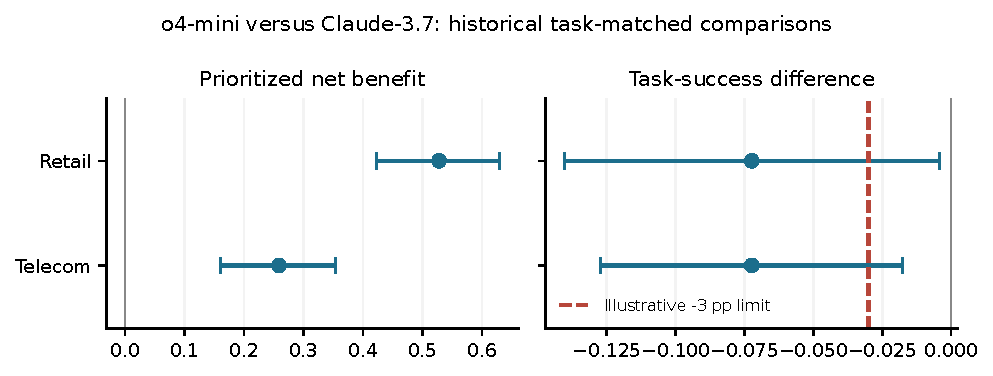
\includegraphics[width=\linewidth]{../results/public_guardrail_reversal.pdf}
\caption{Historical agent comparisons: net benefit and success-rate
difference can favor opposite systems. Intervals are pointwise task
bootstrap summaries, conditional on the archived run configurations;
they do not supply simultaneous or production-population guarantees.}
\label{fig:public}
\end{figure}

The two reversals persist for cost tolerances from 0\% to 20\%. Changing
the priority itself matters: placing tool-call count before cost changes
the telecom o4-mini--Claude-3.7 net benefit from $0.259$ to $-0.126$.
This is a different preference question, not an estimator inconsistency.
SWE-agent Claude-3-Opus versus GPT-4 has net benefit $-0.113$ and success
difference $-0.063$ on the archived runs. These case studies retain
historical model, harness, and price limitations; they do not assert a
ranking of current models.
}{}
\IfFileExists{prospective_results.tex}{\paragraph{Prospective workflow feasibility pilot.}
We froze 12 telecom tasks and compared standard Haiku against the same
model with a verification instruction, with a common Haiku user simulator,
randomized workflow order, deterministic task checks and a 40-step cap.
The fixed monetary stopping rule produced 18/24 completed runs and 9/12
complete pairs; 12 completed runs reached the step cap. Each workflow
succeeded on 2/9 completed tasks. Across all 12 planned tasks, conservative
missing-outcome bounds are $[-0.417,0.083]$ for net preference and
$[-0.25,0.25]$ for success difference (verification minus standard).
These finite-cohort bounds are not sampling intervals. Accounted pilot
cost was \$3.9456 within the frozen \$4 cap. The result demonstrates
execution and measurement feasibility; low success and incomplete pairs
preclude a superiority conclusion. Appendix~\ref{app:pilot} retains the
full cohort, protocol amendment, costs and failure accounting.
}{}
